
\section{Test}

Nella seguente sezione verranno espresse in maniera dettagliata le varie metodologie di test, gli
obiettivi del testing e i criteri di successo utilizzati durante lo sviluppo del prodotto.
Il gruppo SWEet16, durante lo sviluppo dell' RTB, ha eseguito esclusivamente un'unica tipologia di test sui vari componenti utilizzati nella programmazione del PoC. Per perseguire la correttezza del prodotto e facilitare la fase di validazione, la verifica è stata svolta in parallelo allo sviluppo (\emph{Modello a V}$^{G}$).
I test dovranno essere resi il più automatici possibile, per evitare che la fase di testing rallenti la
produzione.

\begin{center}
    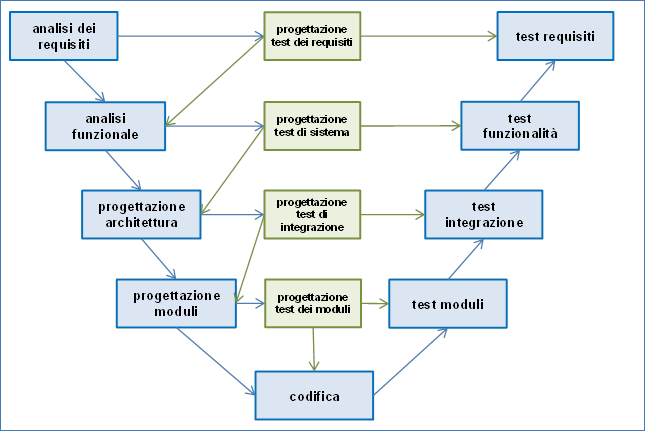
\includegraphics[width=12cm]{test_v.png}
\end{center}
\begin{center}
Immagine 1: Modello a V
\end{center}

\subsection{Tipologie di test}

\subsubsection{Test di unità}

I \textit{test di unità} sono un tipo di test che viene utilizzato per verificare il funzionamento di una singola unità di codice all'interno di un software.
Una unità di codice può essere una funzione, una classe o qualsiasi altra porzione di codice che
svolge una specifica attività all'interno del software.
Questa viene definita con l’inizio del processo di progettazione e sviluppo software.

\subsubsection{Test di integrazione}

I \textit{test di integrazione} sono un tipo di test che viene utilizzato per verificare il funzionamento delle diverse componenti di un software quando vengono integrate tra loro e sono particolarmente utili
per identificare e risolvere eventuali problemi di integrazione.
Inoltre, i \textit{test di integrazione} possono essere utilizzati per verificare che il software soddisfi i requisiti prestabiliti in modo completo e che sia pronto per essere messo in produzione.

\subsubsection{Test di sistema}

I \textit{test di sistema} vengono utilizzati per verificare il funzionamento del software come sistema
completo, inclusi tutti i componenti e le interfacce con gli altri sistemi. I test di sistema hanno lo
scopo di verificare che il software soddisfi i requisiti prestabiliti e che sia pronto per essere messo in
produzione. In particolare, questa tipologia di test mira a soddisfare tutti i requisiti funzionali e la maggior parte di quelli non funzionali, compresi aspetti relativi all’usabilità, sicurezza,
performance e vulnerabilità.

\subsubsection{Test di accettazione}

I \textit{test di accettazione} sono un tipo di test che viene utilizzato per verificare che il software soddisfi i requisiti prestabiliti dal capitolato e che sia pronto per essere consegnato al committente o messo in produzione.
Vengono svolti alla presenza del committente e mirano a soddisfare pienamente i requisiti,
accertandosi di avere un prodotto funzionante e soddisfacente le aspettative progettuali iniziali.

\subsubsection{Test di regressione}

I \textit{test di regressione} sono un tipo di test che viene utilizzato per verificare che le modifiche apportate ad un software non influiscano negativamente sulle sue funzionalità esistenti, sono particolarmente utili per garantire che il software continui a funzionare correttamente anche dopo aver apportato modifiche o aggiornamenti.
Consistono nella ripetizione selettiva di \textit{test di unità, integrazione e sistema}, verificando quindi di non perdere funzionalità nella progressiva realizzazione del prodotto software.


\subsection{Specifica dei test}
Al fine di garantire di creare una denominazione uniforme e per facilitare la comprensione, i test sono identificati da un codice come segue:
\begin{center}
    \textbf{T[Tipologia][Identificativo]}
\end{center}
Dove:
\begin{itemize}
    \item \textbf{Tipologia} indica il tipo del test eseguito:
    \begin{itemize}
        \item U: Per Test di Unità;
        \item I: Per Test di Integrazione;
        \item S: Per Test di Sistema;
        \item A: Per Test di Accettazione;
        \item R: Per Test di Regressione.
    \end{itemize}
    \item \textbf{Identificativo} del test in oggetto.
\end{itemize}
Ciascuna tipologia di test sarà rappresentata da apposite tabelle, comprensive di identificativo, descrizione e stato. Come riportato precedentemente, al momento sono stati effettuati esclusivamente i \textit{test di unità}.

\begin{comment}

    \subsubsection{Test di unità}

\begin{tblr}{
colspec={|X[2.5cm, halign=c]|X[9cm, halign=c]|X[3.5cm, halign=c]|},
row{odd}={bg=white},
row{even}={bg=white},
row{1}={bg=black, fg=white},
}
        Identificativo & Descrizione & Stato \\
        \hline
        TU1 & Si verifica che il componente DashboardClienti venga renderizzato correttamente & Superato \\
        \hline
        TU2 & Si verifica che il componente DashboardRistoratori venga renderizzato correttamente & Superato \\
        \hline
        TU3 & Si verifica che il componente DettagliPietanza venga renderizzato correttamente & Superato \\
        \hline
        TU4 & Si verifica che il componente DettagliPrenotazione venga renderizzato correttamente & Superato \\
        \hline
        TU5 & Si verifica che il componente FormPrenotazione venga renderizzato correttamente & Superato \\
        \hline
        TU6 & Si verifica che il componente MenuPietanze venga renderizzato correttamente & Superato \\
        \hline
        TU7 & Si verifica che il componente Navbar venga renderizzato correttamente & Superato \\
        \hline
        TU8 & Si verifica che il componente Login venga renderizzato correttamente & Superato \\
        \hline
        TU9 & Si verifica che il componente ListaOrdinazioni venga renderizzato correttamente & Superato \\
        \hline
        TU10 & Si verifica che il componente DashboardClienti visualizzi correttamente le prenotazioni del cliente & Superato \\
        \hline
        TU11 & Si verifica che il componente DashboardRistoratori visualizzi correttamente le prenotazioni del ristorante e permetta la loro gestione & Superato \\
        \hline
        TU12 & Si verifica che il componente DettagliPietanza visualizzi correttamente tutti i dettagli della pietanza e permetta l'ordinazione con l'eventuale rimozione di ingredienti & Superato \\
        \hline
        TU13 & Si verifica che il componente DettagliPrenotazione visualizzi correttamente i dettagli di ciascuna prenotazione e ne permetta la gestione & Superato \\
        \hline
        TU14 & Si verifica che il componente FormPrenotazione contsenta correttamente di effettuare una prenotazione & Superato \\
        \hline
        TU15 & Si verifica che il componente MenuPietanze visualizzi correttamente tutto il menù e permette l'ordinazione di ciascuna pietanza & Superato \\
        \hline
\end{tblr}

\begin{tblr}{
colspec={|X[2.5cm, halign=c]|X[9cm, halign=c]|X[3.5cm, halign=c]|},
row{odd}={bg=white},
row{even}={bg=white},
}
        \hline
        TU16 & Si verifica che il componente Navbar visualizzi correttamente la pagina attuale, le altre pagine e il nome dell'utente o del ristoratore loggato & Superato \\
        \hline
        TU17 & Si verifica che il componente Login permetta correttamente di effettuare l'accesso tramite cliente o ristoratore & Superato \\
        \hline
        TU18 & Si verifica che il componente ListaOrdinazioni visualizzi correttamente le ordinazioni confermate e l'inventario degli ingredienti & Superato \\
        \hline

\end{tblr}

\end{comment}
